\section{Theorie}
\label{sec:Theorie}

\subsection{Röntgenemissionsspektrum}
\label{sec:Theorie_emission}

Zur Erzeugung von Röntgenstrahlung werden in einer evakuierten Röhre durch eine
Glühkathode Elektronen freigesetzt. Diese werden durch eine sehr hohe Spannung zu
einer Anode hin stark beschleunigt. Beim Auftreffen der Elektronen auf die Anode
entsteht Röntgenstrahlung. Diese besteht aus der kontinuierlichen Bremsstrahlung
und der für das Material der Anode spezifischen und diskreten charakteristischen
Strahlung.

Das Bremsspektrum, das in Abbildung \ref{fig:bremsspektrum} skizziert ist, entsteht
durch das Abbremsen der Elektronen auf der Anode durch Coulombwechselwirkung. Dabei
wird ein Photon ausgesandt, das genau die Energie besitzt, die das Elektron durch
diesen Abbremsvorgang verliert. Das Elektron muss dabei nicht zwangsläufig völlständig
abgebremst werden, gibt also nicht in jedem Fall seine gesamte Energie ab. Aufgrunddessen
ist das Spektrum kontinuierlich. Das Spektrum hat jedoch eine untere Grenze $\lambda_{\symup{min}}$
für die Wellenlänge. Diese folgt dem Zusammenhang
\begin{equation}
  \lambda_{\symup{min}}=\frac{hc}{e_0 U} \,.
\end{equation}
Die Photonen mit dieser Wellenlänge besitzen die gesamte kinetische Energie eines
Elektrons nun in Form von Stahlungsenergie.

\begin{figure}
  \centering
  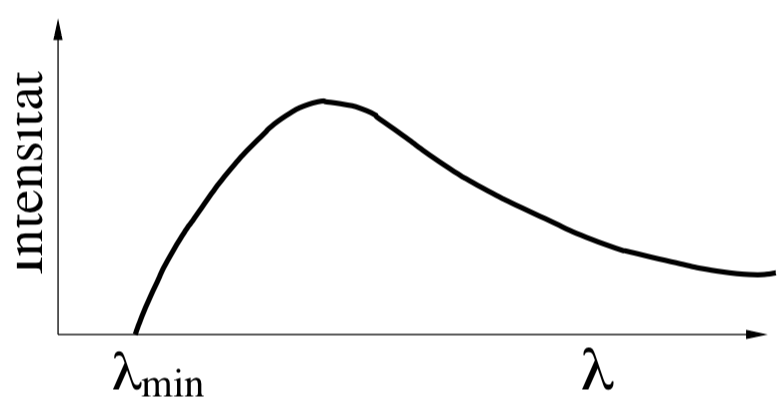
\includegraphics[height=4cm]{data/bremsspektrum.png}
  \caption{Skizze des kontinuierlichen Bremsspektrums \cite{Versuchsanleitung}.}
  \label{fig:bremsspektrum}
\end{figure}

Die charakteristische Stahlung entsteht dadurch, dass die hochenergetischen Elektronen
die Atome der Anode ionisieren, sodass in einer inneren Schale eine Leerstelle entsteht.
In diese Leerstelle kann nun ein Elektron von einer höheren Schale fallen. Da die
Energieniveaus auf den Schalen jedoch nicht identisch sind, wird bei diesem Vorgang
ein Photon ausgesandt, dass als Energie die Energiedifferenz der beiden Schalen besitzt:
\begin{equation}
  hf=E_{\symup{m}}-E_{\symup{n}} \,.
\end{equation}
Diese Energiedifferenzen sind charakteristisch für das Anodenmaterial.

In einem Atom mit mehreren Elektronen wird die Kernladung durch die Elektronen
abgeschirmt. Damit wird die Coulomb-Kraft auf ein Elektron auf der n-ten Schale auf
\begin{equation}
  E_{\symup{n}}=-R_{\symup{\infty}} z_{\symup{eff}}^2 \cdot \frac{1}{n^2}
\end{equation}
reduziert. Dabei ist $R_{\symup{\infty}}=13.6\,$eV die Rydbergenergie und
$z_{\symup{eff}}=z-\sigma$ die effektive Kernladung, wobei $\sigma$ die
Abschirmkonstante ist.

Jede charakteristische Linie besteht aus mehreren eng beieinanderliegenden Linien.
Dies nennt man auch die Feinstruktur der charakteristischen Strahlung. Diese tritt auf,
da die äußeren Elektronen aufgrund von Spins und Bahndrehimpulsen leicht unterschiedliche
Bindungsenergien besitzen. Diese Bindungsenergie beschreibt die Sommerfeld'sche
Feinstrukturformel:
\begin{equation}
  E_{\symup{n,j}}=-R_{\symup{\infty}}\Biggl(z_{\symup{eff,1}}^2\cdot \frac{1}{n^2} +
   \alpha^2 z_{\symup{eff,2}}^4\cdot \frac{1}{n^3}\Biggl(\frac{1}{j+\frac{1}{2}} -
   \frac{3}{4n}\Biggr)\Biggr) \,.
\end{equation}
$R_{\symup{\infty}}$ ist hier erneut die Rydbergenergie und $z_{\symup{eff}}$ erneut
die effektive Kernladungszahl. $\alpha$ ist die Sommerfeld'sche Konstante, $n$
die Hauptquantenzahl und $j$ der Bahndrehimpuls des Elektrons.

\subsection{Röntgenabsorptionsspektrum}
\label{sec:Theorie_absorption}


\begin{figure}
  \centering
  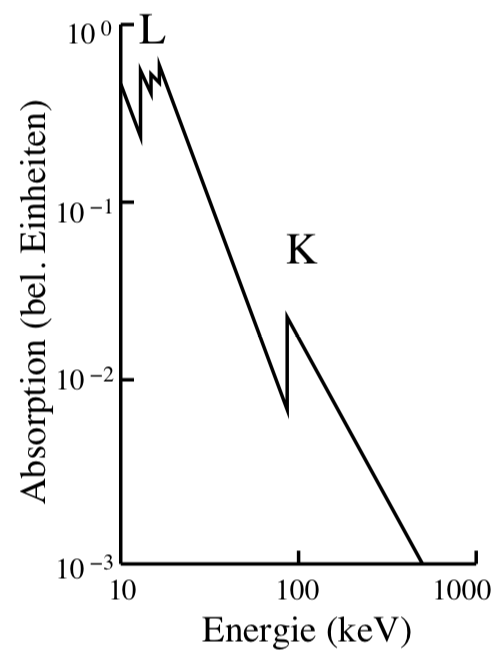
\includegraphics[height=4cm]{data/absorption.png}
  \caption{Skizze des Absorptionsspektrums \cite{Versuchsanleitung}.}
  \label{fig:absorption}
\end{figure}
